\documentclass{article}

% MATHS
\usepackage{amsmath}
\usepackage{gensymb}

\usepackage{mathtools}
\newcommand\coolover[2]{\mathrlap{\smash{\overbrace{\phantom{%
    \begin{matrix} #2 \end{matrix}}}^{\mbox{$#1$}}}}#2} 
\newcommand\coolunder[2]{\mathrlap{\smash{\underbrace{\phantom{%
    \begin{matrix} #2 \end{matrix}}}_{\mbox{$#1$}}}}#2}
    
\newcommand\coolleftbrace[2]{%
#1\left\{\vphantom{\begin{matrix} #2 \end{matrix}}\right.}

\newcommand\coolrightbrace[2]{%
\left.\vphantom{\begin{matrix} #1 \end{matrix}}\right\}#2}


% GRAPHICS
\usepackage{float}
\usepackage{subcaption}
\usepackage{tikz}
\usepackage{tikzscale}
\usetikzlibrary{calc}
\usepackage{graphicx}

% HYPERLINKS
\usepackage{hyperref}

% DOCUMENT PADDING AND MARGINS
\usepackage{titlesec}
\usepackage[margin=1.2in]{geometry}
\setlength{\parskip}{\baselineskip}%
\setlength{\parindent}{0pt}
\titlespacing*{\section}{0pt}{5ex}{2ex}
\titlespacing*{\subsection}{0pt}{1ex}{-2ex}
\titlespacing*{\subsubsection}{0pt}{2ex}{-2ex}

%COMMENTING
\usepackage{comment}


\begin{document}

% TITLE
\title{ME780 Assignment 1}
\author{Stan Brown \& Chris Choi}
\date{}
\maketitle



\section{Derivation of the Omni-directional Robot}
\label{sec:motion_model_derivation}

\begin{figure}[H]
	\centering
	\begin{subfigure}[b]{0.45\linewidth}
		\includegraphics[width=\textwidth]{images/omni_robot_1.tikz}
		\caption{Omni-Directional Robot in Body Frame}
	\end{subfigure}
	\begin{subfigure}[b]{0.45\linewidth}
		\includegraphics[width=\textwidth]{images/omni_robot_2.tikz}
		\caption{Body Frame w.r.t Each Wheel}
	\end{subfigure}
	\caption{Omni-Directional Robot}
	\label{fig:omni_robot}
\end{figure}


Here we derive the kinematics of the Omni-directional robot. We followed the
generalized approach in \cite{Siegwart04} in resolving how each wheel
contributes to the robot chassis. The generalized equation is:

\begin{equation}
	\label{eq:general_robot_kinematics_equation}
    \xi_{I} = R(\theta)^{-1} J_{1}^{-1} J_{2} \omega
\end{equation}

Where:

\begin{itemize}
	\vspace{-0.4cm}
	\setlength{\itemsep}{0pt}
	\setlength{\parskip}{0pt}
	\setlength{\parsep}{0pt}
	
    \item{$\xi_{I}$: State in the body frame}
    \item{$R(\theta)$: Rotation matrix}
    \item{$J_{1}$: Wheel constraints}
    \item{$J_{2}$: Diagonal matrix denoting the radii $r$ of each wheel}
    \item{$\omega$: Angular velocity $\omega$ of each wheel}
\end{itemize}

\newpage
Deriving the robot kinematics for each wheel we get in the form of 
\ref{eq:general_robot_kinematics_equation} we obtain:

\begin{align}
	\vphantom{% phantom stuff for correct box dimensions
    \begin{matrix}
    	\overbrace{XYZ}^{\mbox{$R$}} \\ \\
    	\underbrace{pqr}_{\mbox{$S$}}
    \end{matrix}}%
	J_{1} &= 
	\begin{bmatrix}
			0 & 1 & l \\
  	    	-\cos(\frac{\pi}{6}) & -\sin(\frac{\pi}{6}) & l \\
   	    	\cos(\frac{\pi}{6}) & -\sin(\frac{\pi}{6}) & l
    \end{bmatrix}
    \begin{matrix}% matrix for right braces 
        \coolrightbrace{x}{Wheel 1}\\
	    \coolrightbrace{x}{Wheel 2}\\
	    \coolrightbrace{x}{Wheel 3}
    \end{matrix} \\
    J_{2} &=
    \begin{bmatrix}
        r & 0 & 0 \\
        0 & r & 0 \\
        0 & 0 & r
    \end{bmatrix} \\
    \omega &= 
	    \begin{bmatrix}
	       \omega_{1} \\
	       \omega_{2} \\
	       \omega_{3} \\
	    \end{bmatrix}
\end{align}

Putting it all together we have:

\begin{align}
	\vspace{-0.4cm}
    \xi_{I}
        &= R(\theta)^{-1} J_{1}^{-1} J_{2} \omega \\
    \begin{bmatrix}
        \dot{x} \\
        \dot{y} \\
        \dot{\theta}
    \end{bmatrix}      
        &= 
        \begin{bmatrix}
	        \cos{(\theta)} & -\sin{(\theta)} & 0 \\
	        \sin{(\theta)} & \cos{(\theta)} & 0 \\
	        0 & 0 & 1
        \end{bmatrix}^{-1}
        \begin{bmatrix}
            0 & 1 & l \\
          	-\cos(\frac{\pi}{6}) & -\sin(\frac{\pi}{6}) & l \\
        	\cos(\frac{\pi}{6}) & -\sin(\frac{\pi}{6}) & l
        \end{bmatrix}^{-1}
        \begin{bmatrix}
            r & 0 & 0 \\
            0 & r & 0 \\
            0 & 0 & r
        \end{bmatrix}
	    \begin{bmatrix}
	       \omega_{1} \\
	       \omega_{2} \\
	       \omega_{3} \\
	    \end{bmatrix} \\
	 \begin{bmatrix}
	     \dot{x} \\
	     \dot{y} \\
	     \dot{\theta}
	 \end{bmatrix} 
	 	&=
		\begin{bmatrix}
			\cos{(\theta)} & \sin{(\theta)} & 0 \\
			-\sin{(\theta)} & \cos{(\theta)} & 0 \\
			0 & 0 & 1
		\end{bmatrix}
		\begin{bmatrix}
			0 & -\frac{1}{\sqrt{3}} & \frac{1}{\sqrt{3}} \\
			\frac{2}{3} & -\frac{1}{3} & -\frac{1}{3} \\
			\frac{1}{3l} & \frac{1}{3l} & \frac{1}{3l}
		\end{bmatrix}
		\begin{bmatrix}
			r & 0 & 0 \\
			0 & r & 0 \\
			0 & 0 & r
		\end{bmatrix}
	    \begin{bmatrix}
	       \omega_{1} \\
	       \omega_{2} \\
	       \omega_{3} \\
	    \end{bmatrix} \\
	\begin{bmatrix}
		\dot{x} \\
		\dot{y} \\
		\dot{\theta}
	\end{bmatrix} 
		&=
		\begin{bmatrix}
			\frac{2}{3} \sin(\theta) 
				& -\frac{1}{\sqrt{3}} \cos(\theta) 
					-\frac{1}{3} \sin(\theta)
				& \frac{1}{\sqrt{3}} \cos(\theta) 
					-\frac{1}{3} \sin(\theta) \\
			\frac{2}{3} \cos(\theta)
				& \frac{1}{\sqrt{3}} \sin(\theta) 
					-\frac{1}{3} \cos(\theta)
				& -\frac{1}{\sqrt{3}} \sin(\theta) 
					-\frac{1}{3} \cos(\theta) \\
			\frac{1}{3l} 
				& \frac{1}{3l}
				& \frac{1}{3l}
		\end{bmatrix}
		\begin{bmatrix}
			r \omega_{1} \\
			r \omega_{2} \\
			r \omega_{3} \\
		\end{bmatrix} \\
	\begin{bmatrix}
		\dot{x} \\
		\dot{y} \\
		\dot{\theta}
	\end{bmatrix} 
		&=
		\begin{bmatrix}
			\frac{2}{3} \sin(\theta) r \omega_{1}
				- \frac{1}{\sqrt{3}} \cos(\theta) r \omega_{2}
					- \frac{1}{3} \sin(\theta) r \omega_{2}
				+ \frac{1}{\sqrt{3}} \cos(\theta) r \omega_{3}
					- \frac{1}{3} \sin(\theta) r \omega_{3} \\
			\frac{2}{3} \cos(\theta) r \omega_{1}
				+ \frac{1}{\sqrt{3}} \sin(\theta) r \omega_{2}
					-\frac{1}{3} \cos(\theta)r \omega_{2}
				- \frac{1}{\sqrt{3}} \sin(\theta) r \omega_{3}
					-\frac{1}{3} \cos(\theta) r \omega_{3} \\
			\frac{1}{3l} r \omega_{1}
				+ \frac{1}{3l} r \omega_{2}
				+ \frac{1}{3l} r \omega_{3}
		\end{bmatrix} \\
	\vspace{-0.4cm}
\end{align}

\begin{equation}
	\vspace{-0.4cm}
	\dot{g}(\theta, \omega) 
		= 
		\begin{bmatrix}
			\dot{x} \\
			\dot{y} \\
			\dot{\theta}
		\end{bmatrix} 
\end{equation}

Where: 

\begin{itemize}
	\vspace{-0.4cm}
	\setlength{\itemsep}{0pt}
	\setlength{\parskip}{0pt}
	\setlength{\parsep}{0pt}
	
	\item{$\dot{g}$ is our velocity motion model of the omni-directional robot}
	\item{$\theta$ is the angle (or bearing) of the robot in the inertia frame.}
	\item{$\omega$ is the wheel inputs of the robot 
		$\begin{bmatrix}
			\omega_{1} \\ 
			\omega_{2} \\ 
			\omega_{3}
		\end{bmatrix}$
	}
\end{itemize}






\newpage
\section{Applying the Derived Robot Model}
\label{sec:applying_motion_model}



\subsection{Predefined Rotation Inputs}
\label{subsec:traverse_inputs}
Applying the following rotation inputs to the wheel for 15 seconds:

\begin{itemize}
	\vspace{-0.4cm}
	\setlength{\itemsep}{0pt}
	\setlength{\parskip}{0pt}
	\setlength{\parsep}{0pt}
	
	\item{$\omega_{1} = -15.5 \text{ rad} s^{-1}$}
	\item{$\omega_{2} = 10.5 \text{ rad} s^{-1}$}
	\item{$\omega_{3} = 1.5 \text{ rad} s^{-1}$}
	
	\vspace{-0.4cm}
\end{itemize}

We obtain the following motion.

\begin{figure}[H]
	\centering
	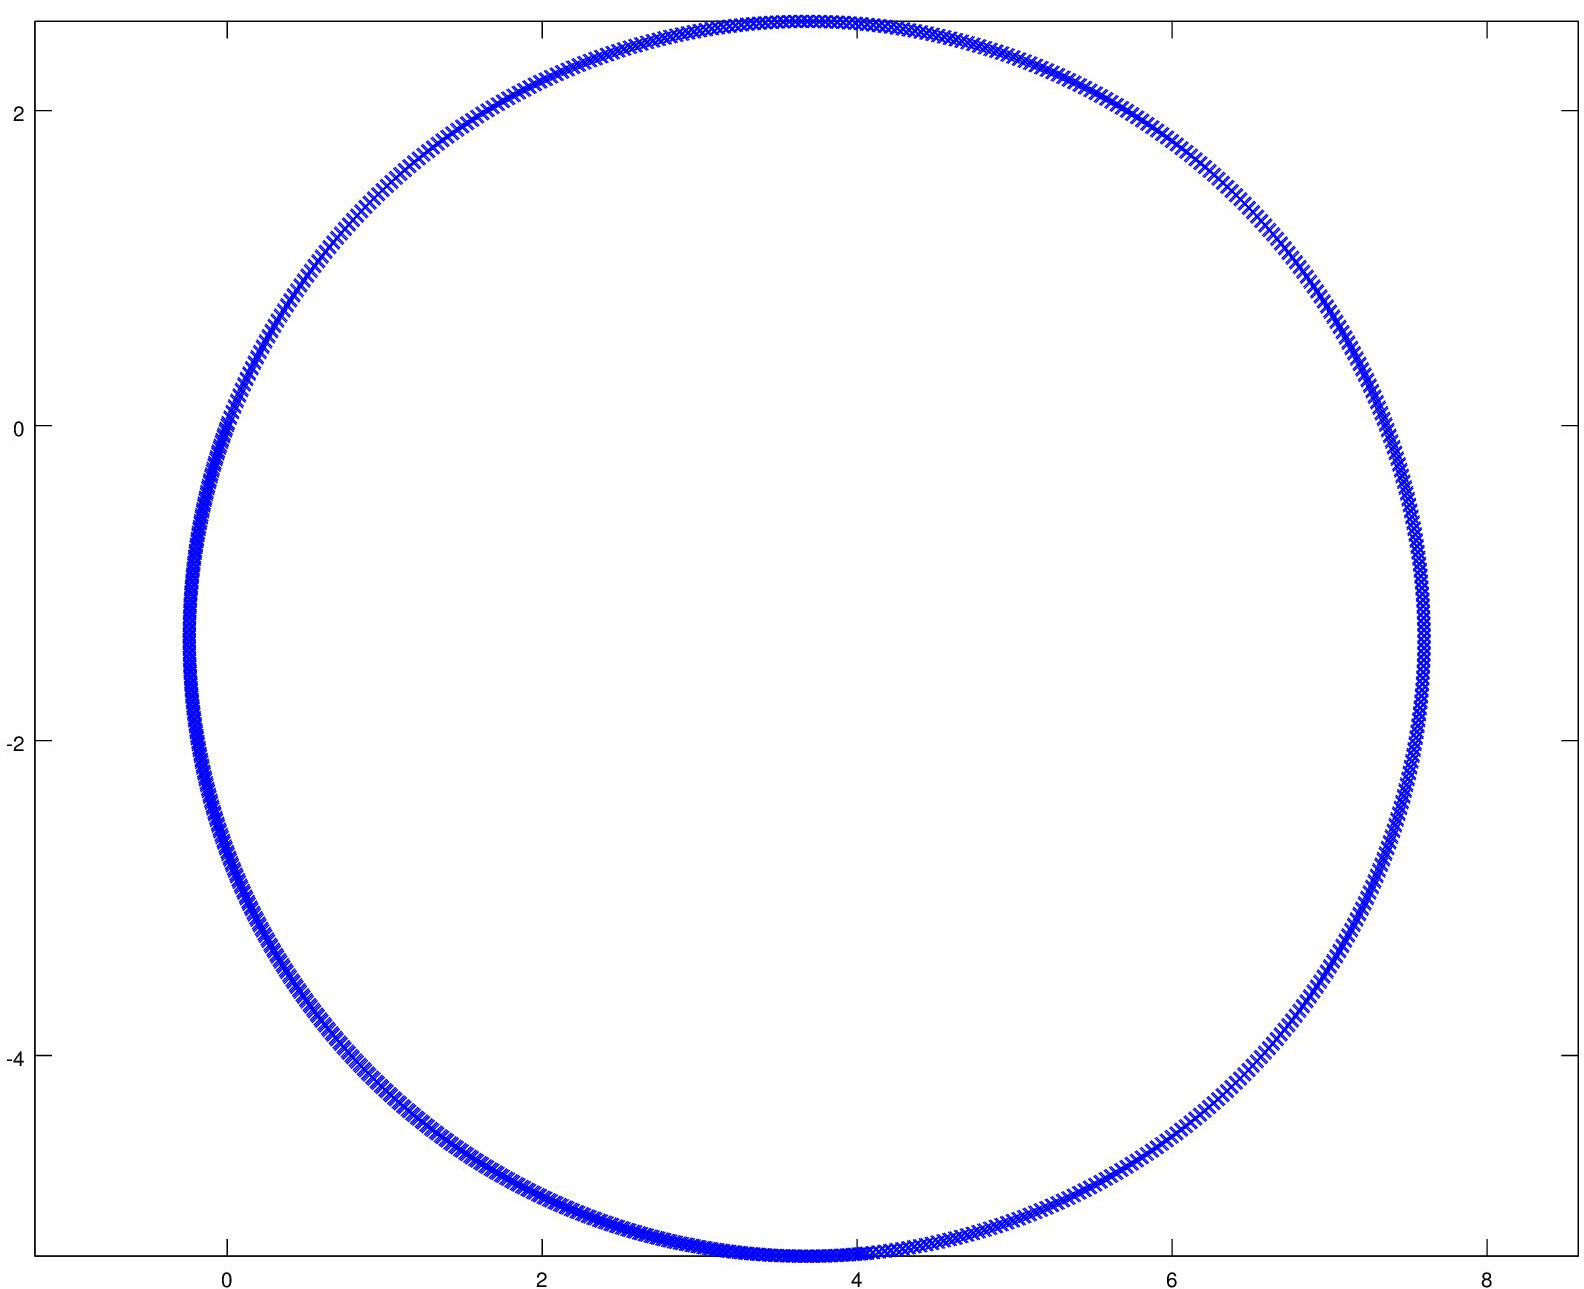
\includegraphics[width=0.5\textwidth]{images/traverse_predefined.jpg}
	\caption{Traverse with inputs:
		$\omega_{1} = -15.5 \text{ rad} s^{-1}$
		$\omega_{2} = 10.5 \text{ rad} s^{-1}$
		$\omega_{3} = 1.5 \text{ rad} s^{-1}$
	}
	\label{fig:omni_robot_predefined}
\end{figure}



\subsection{Traversing East, West, North East, South East and Inplace}
\label{subsec:traverse_directions}

\begin{figure}[H]
	\centering
	
	\begin{subfigure}[b]{0.32\linewidth}
		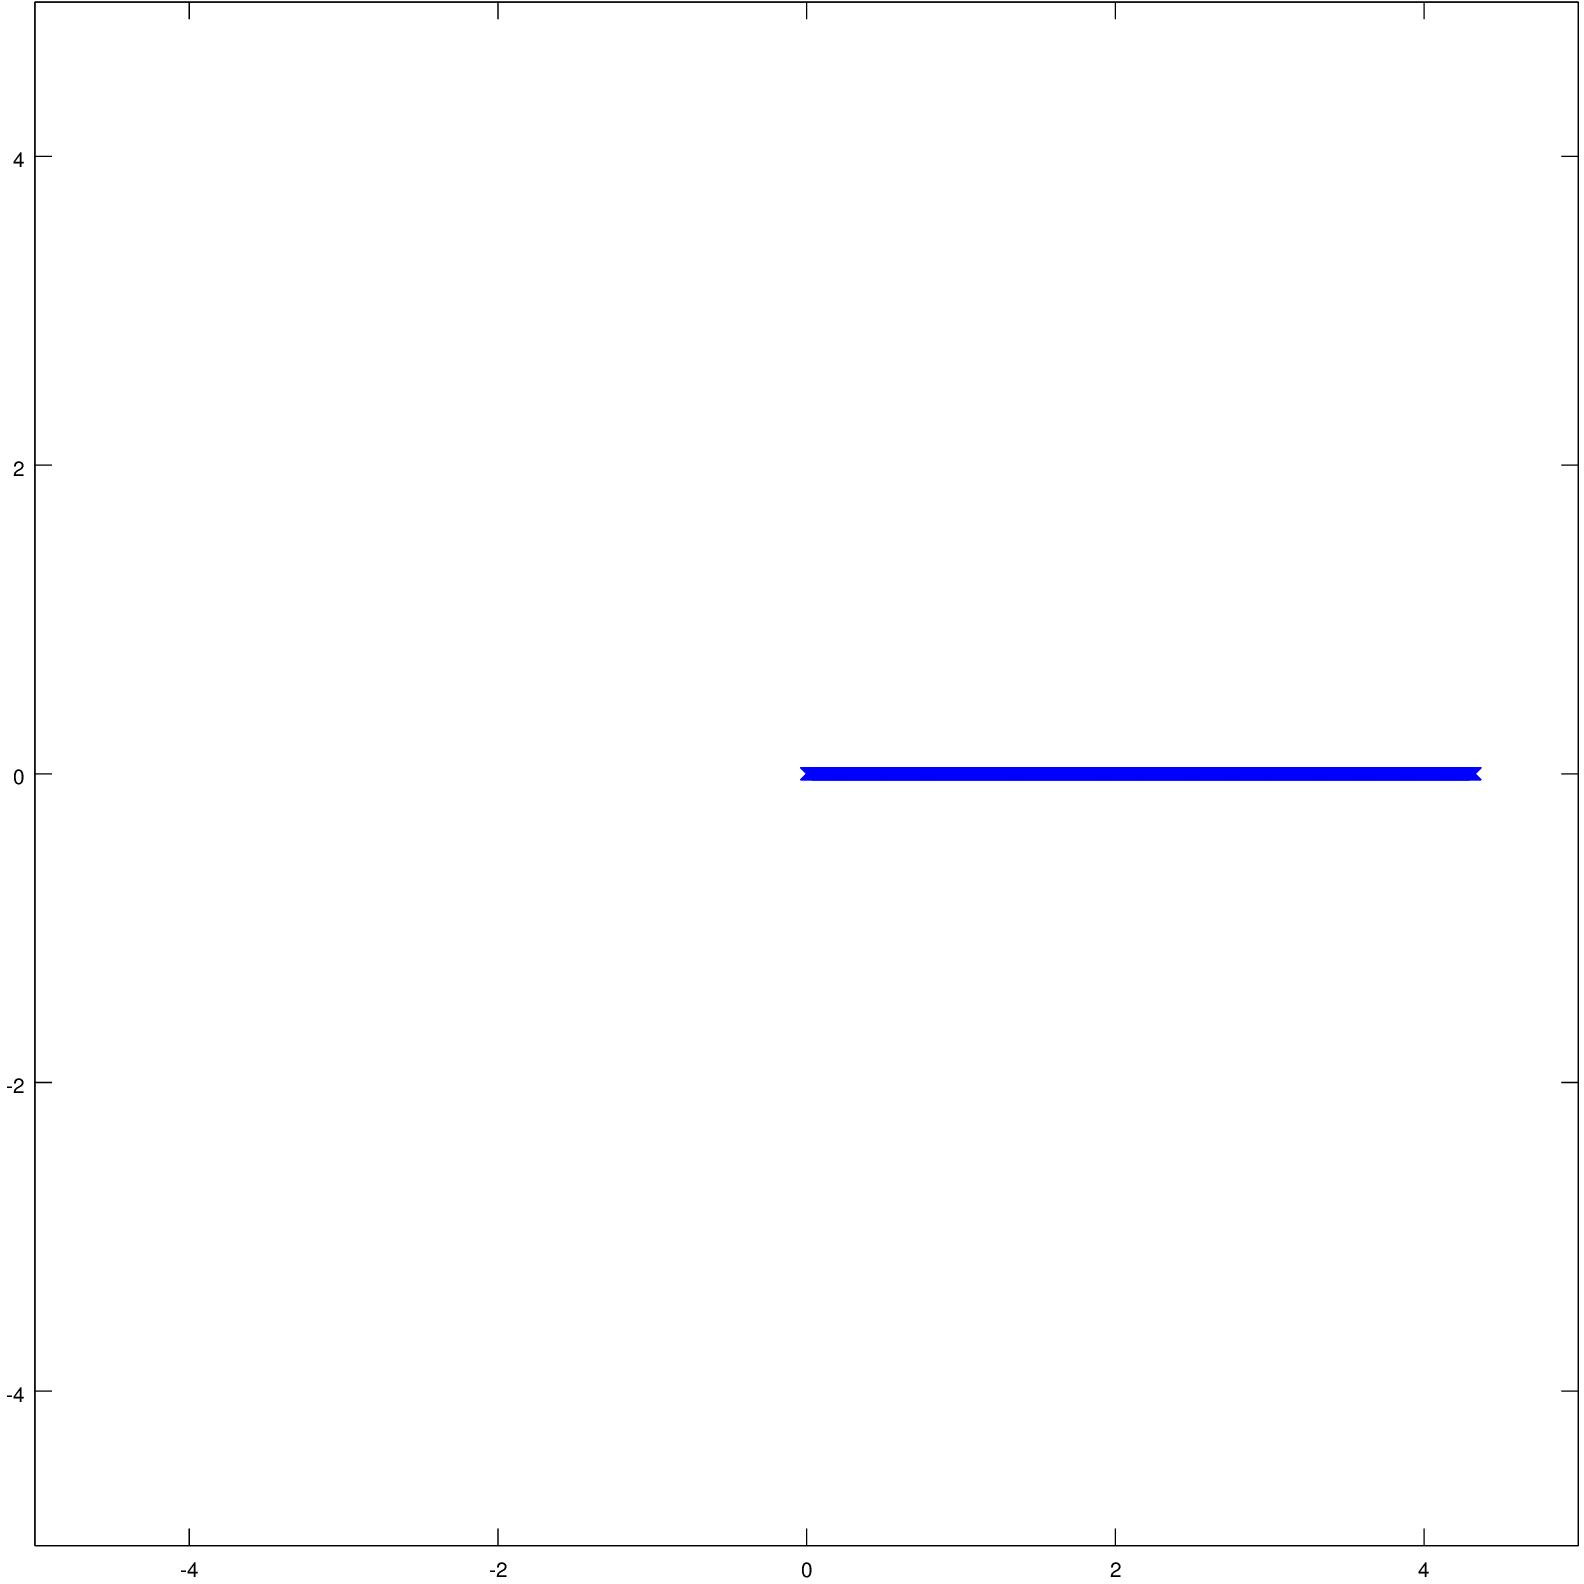
\includegraphics[width=\textwidth]{images/traverse_east.jpg}
		\caption{Traverse East}
	\end{subfigure}
	\begin{subfigure}[b]{0.32\linewidth}
		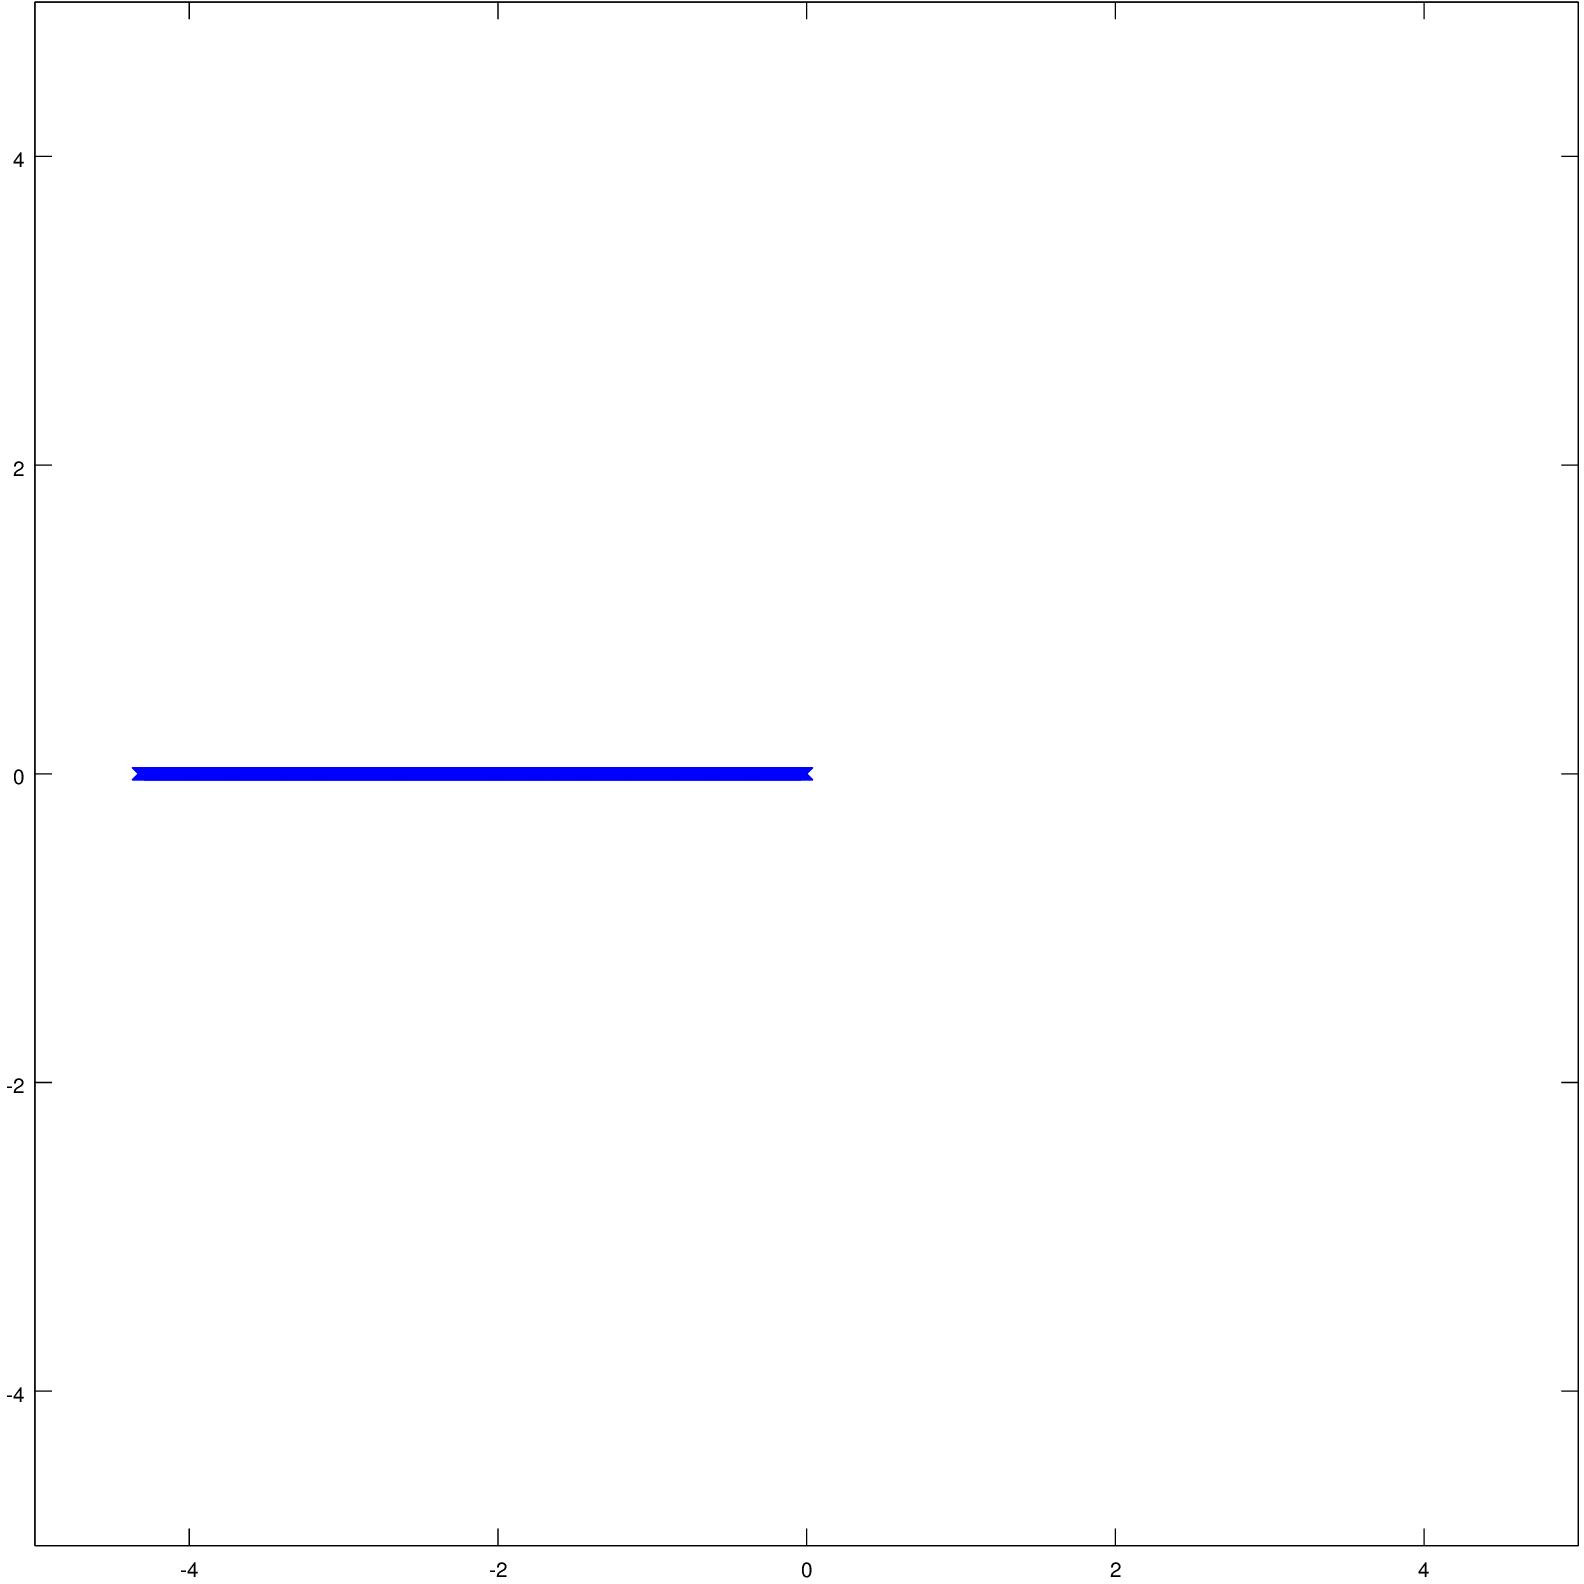
\includegraphics[width=\textwidth]{images/traverse_west.jpg}
		\caption{Traverse West}
	\end{subfigure}
	\begin{subfigure}[b]{0.32\linewidth}
		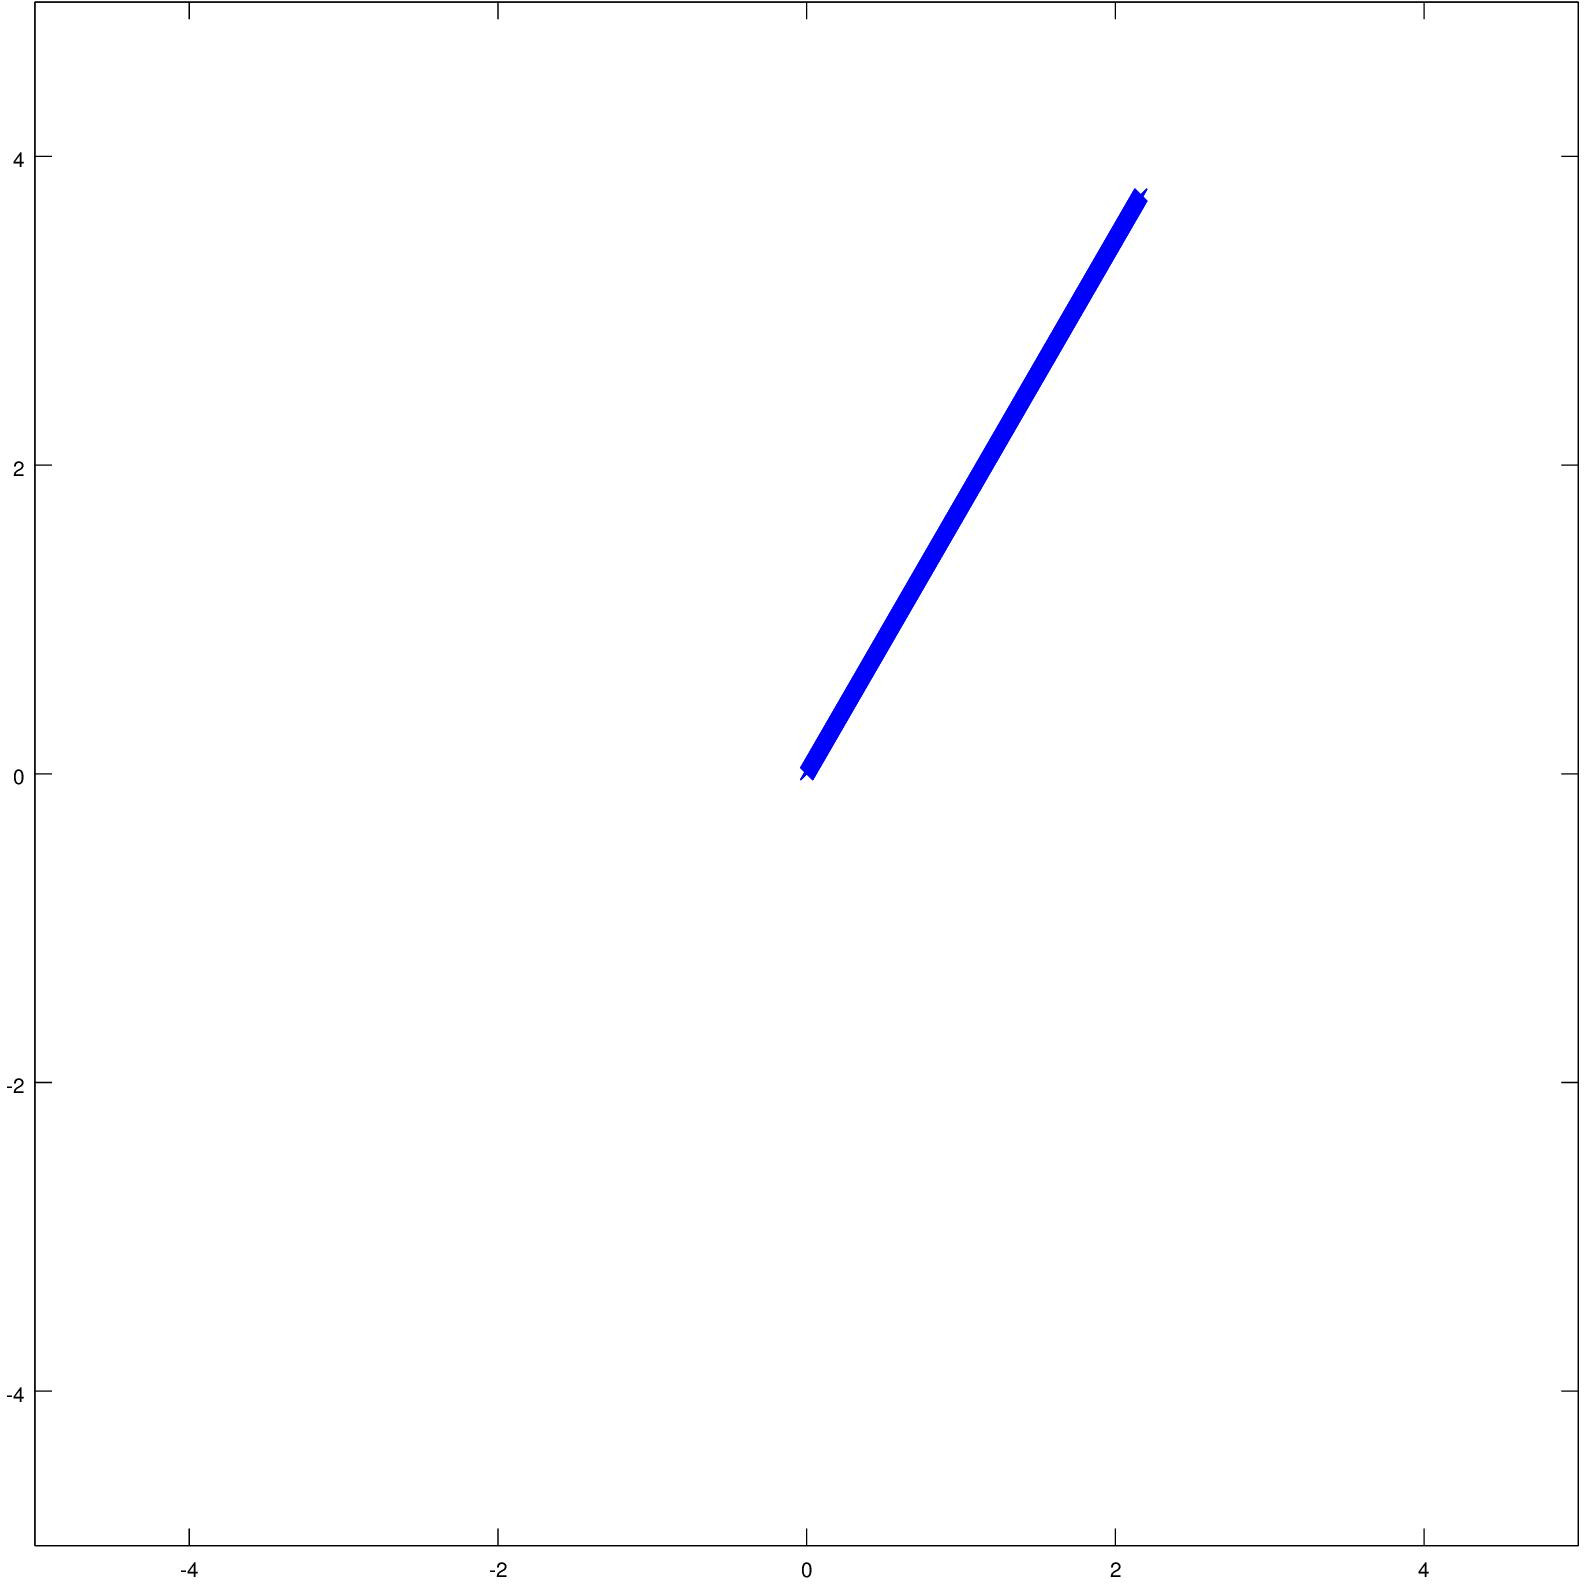
\includegraphics[width=\textwidth]{images/traverse_north_east.jpg}
		\caption{Traverse North East}
	\end{subfigure}
	
	\begin{subfigure}[b]{0.32\linewidth}
		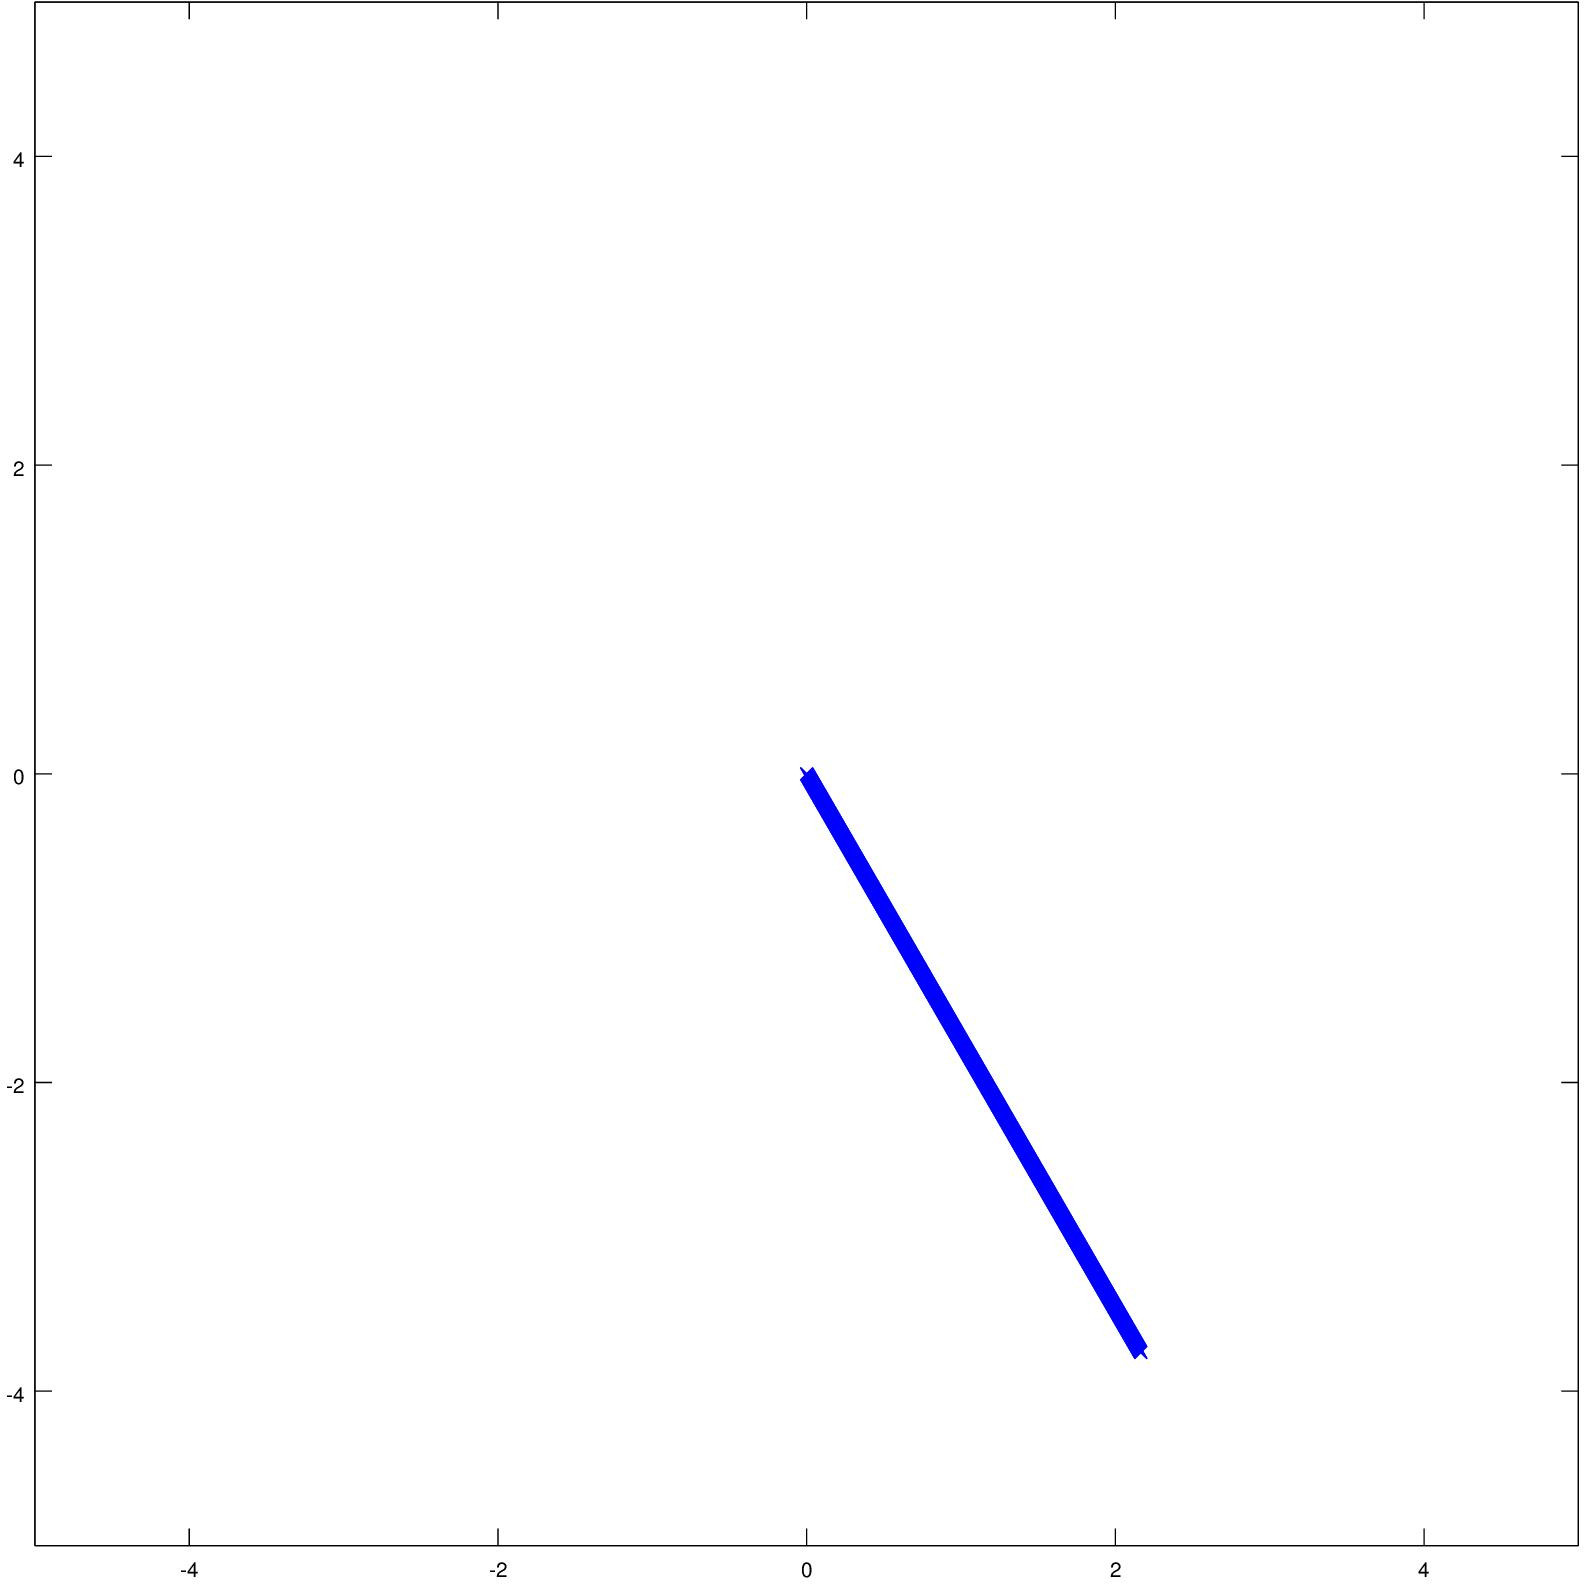
\includegraphics[width=\textwidth]{images/traverse_south_east.jpg}
		\caption{Traverse South East}
	\end{subfigure}
	\begin{subfigure}[b]{0.32\linewidth}
		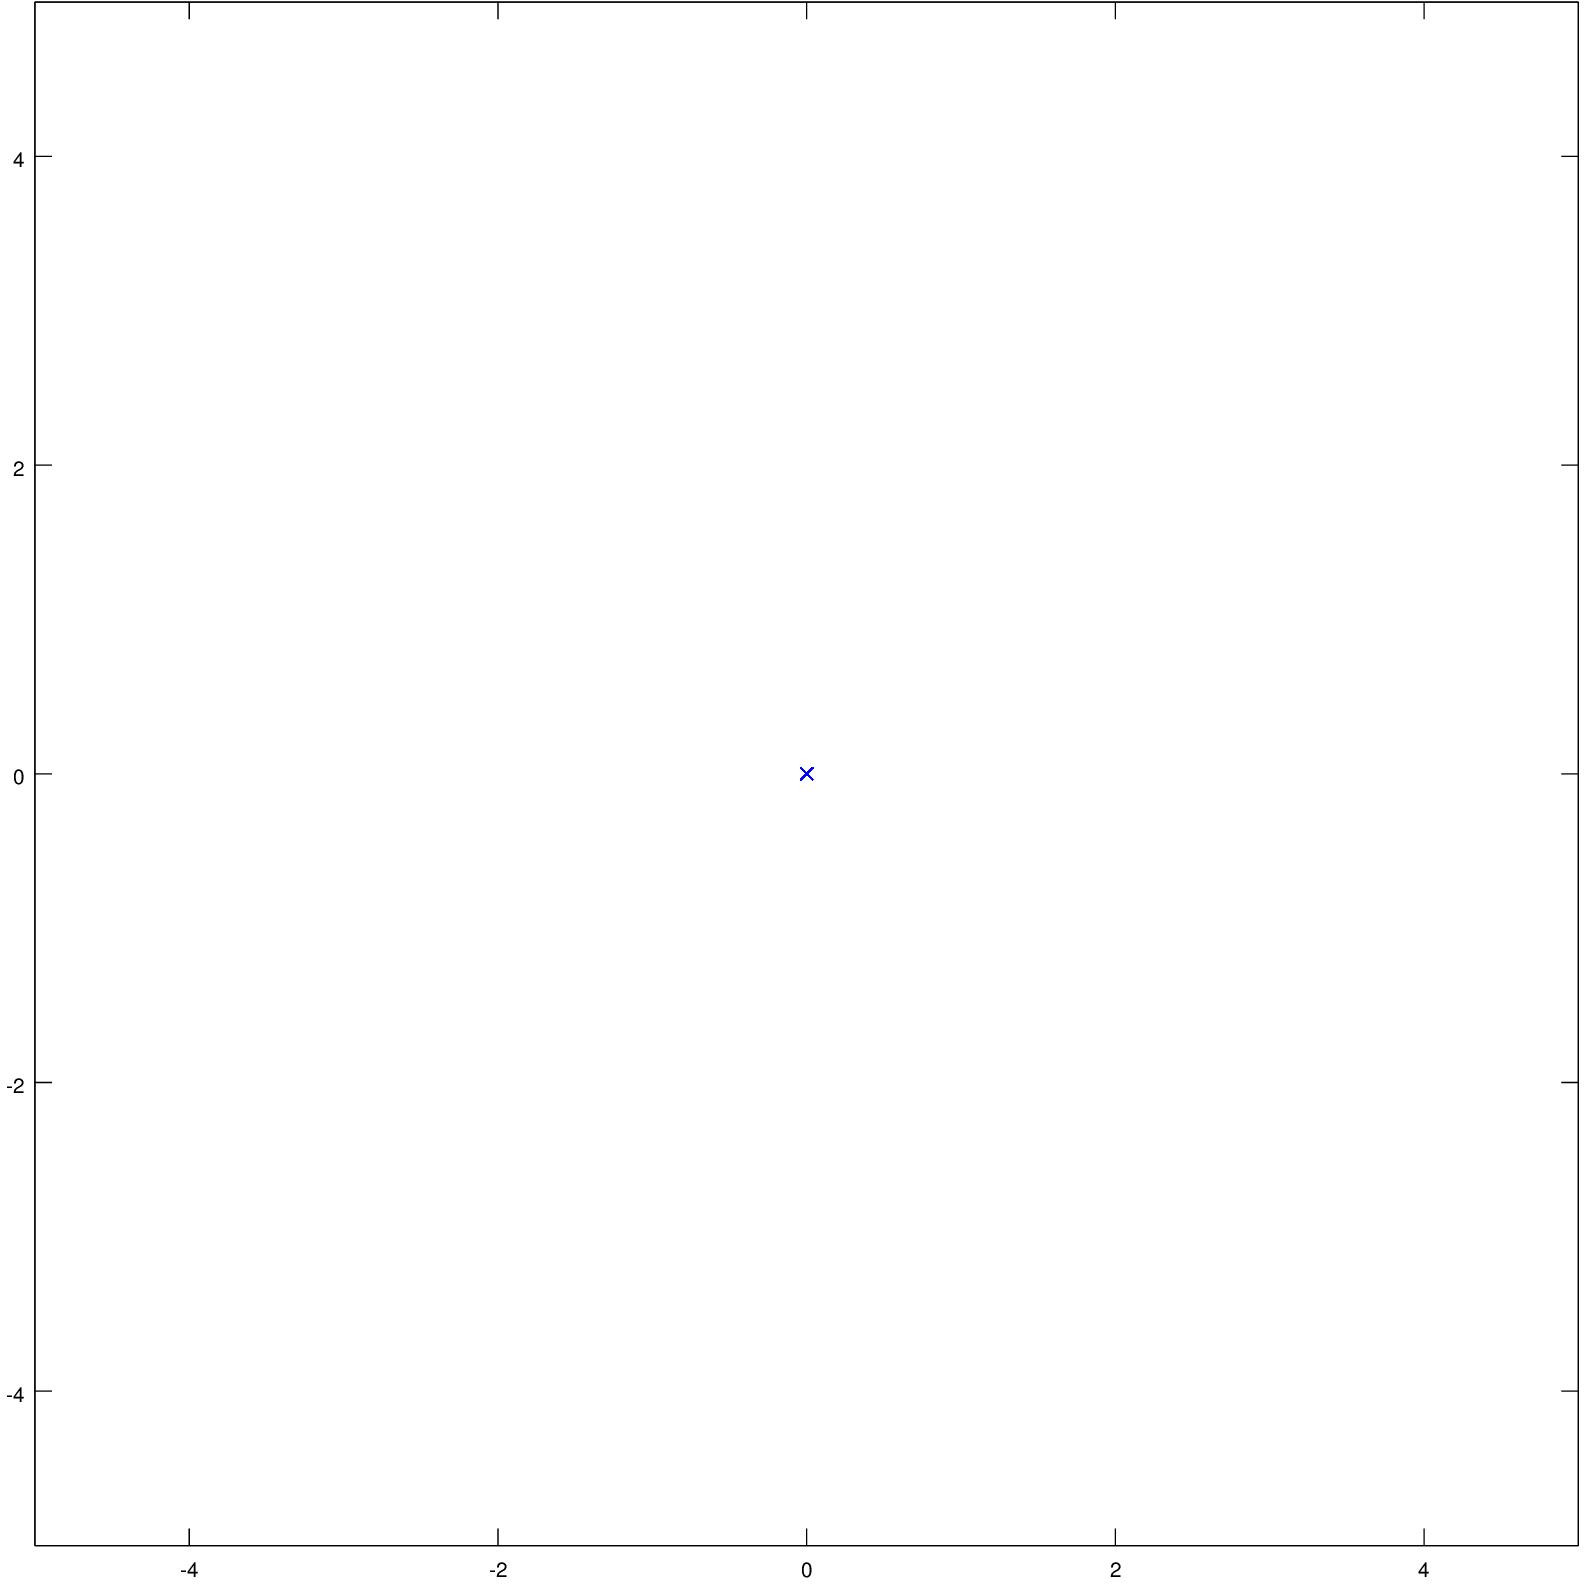
\includegraphics[width=\textwidth]{images/traverse_inplace.jpg}
		\caption{Traverse Inplace}
	\end{subfigure}
	
	\caption{Traversing East, West, North East, South East and Inplace}
	\label{fig:omni_robot_traverse}
\end{figure}

The inputs that drove the robot to traverse in the directions shown in 
Fig~\ref{fig:omni_robot_traverse} for 15 seconds  are as follows:


\begin{itemize}
	\vspace{-0.4cm}
	\setlength{\itemsep}{0pt}
	\setlength{\parskip}{0pt}
	\setlength{\parsep}{0pt}
	
	\item{
		\text{East}: 
		$\omega_{1} = 0$, $\omega_{2} = -1$, $\omega_{3} = 1$
	}
	\item{
		\text{West}: 
		$\omega_{1} = 0$, $\omega_{2} = 1$, $\omega_{3} = -1$
	}
	\item{
		\text{North East}: 
		$\omega_{1} = 1$, $\omega_{2} = -1$, $\omega_{3} = 0$
	}
	\item{
		\text{South East}: 
		$\omega_{1} = -1$, $\omega_{2} = 0$, $\omega_{3} = 1$
	}
	\item{
		\text{Inplace}: 
		$\omega_{1} = 1$, $\omega_{2} = 1$, $\omega_{3} = 1$
	}
\end{itemize}



\newpage
\subsection{Moving in a Circle}
\label{subsec:traverse_circle}

To traverse in a circle of diameter of $2$m, we had to be a little creative
with the rotation inputs of the wheels. To do this we applied the following 
intuition:

\begin{enumerate}
	\vspace{-0.4cm}
	
    \item{Constrained the robot's $y$-axis movement to $0$, 
    and so $\dot{y}$ is $\dot{y} = 0$. Use wheels 2 and 3 as fixed wheels 
    pushing the robot forward, and use wheel 1 as a steering wheel. (See 
    fig~\ref{fig:omni_robot})}

    \item{For the robot to traverse a circle, the robot must traverse the
    circumference of a circle, i.e. $2 \pi R$, where $R$ is the radius of the 
    circle we want the robot to make $d = 2 \pi R$. Converting that to 
    velocity, the equation becomes $\dot{x} = \frac{2 \pi R}{t}$}

    \item{For the robot to make a full circle, it must change angle $\theta = 2 
    \pi$. Converting this to the angular rate the equation becomes 
    $\theta = \frac{2 \pi}{t}$}
    
   	\vspace{-0.4cm}
\end{enumerate}

Putting the above all together we have the following, originally we had:

\begin{equation}
    \xi_{I} = R(\theta)^{-1} J_{1}^{-1} J_{2} \omega
\end{equation}

Where we are trying to figure out what the $\omega$ inputs are to drive the 
robot to make a full circle in the inertial frame, we already know what 
$R(\theta)$, $J_{1}$, $J_{2}$ are, the only unknown left is $\xi_{I}$, but 
using the above intuition we can relate what it should be to make a circle.

\begin{equation}
    \omega = \xi_{I} R(\theta) J_{1} J_{2}^{-1}
\end{equation}

\begin{equation}
    \xi_{I} =
  		\begin{bmatrix}
            \dot{x} \\
            \dot{y} \\
            \dot{\theta}
        \end{bmatrix} 
        =
  		\begin{bmatrix}
            \frac{2 \pi R}{t} \\
            0 \\
            \frac{2 \pi}{t}
        \end{bmatrix}
\end{equation}

Using the above equation we found the $\omega$ inputs required to traverse a 
2m diameter circle in 15 seconds is $\omega_{1} = 0.50265$, $\omega_{2} = 
-0.94838$ $\omega_{3} = 1.95369$ starting from the origin $(0, 0)$.

\begin{figure}[H]
	\centering
	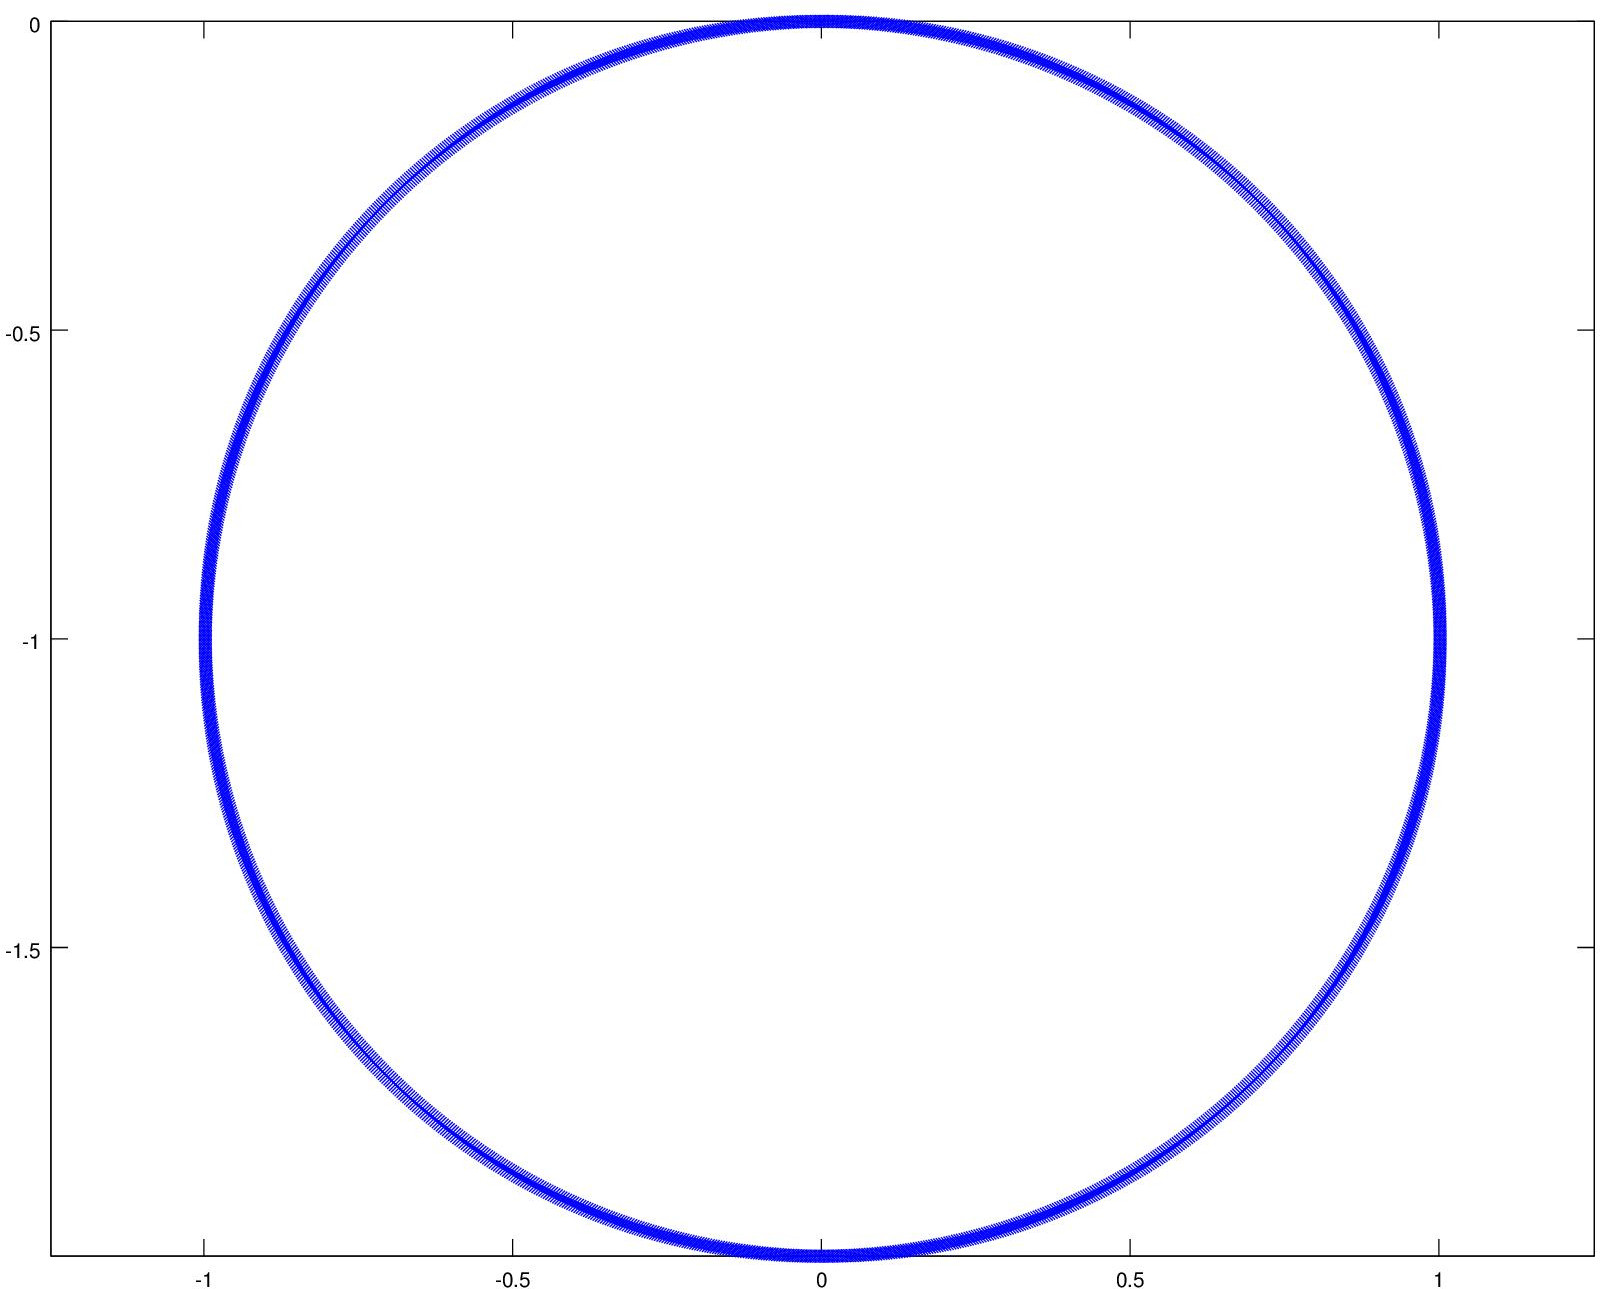
\includegraphics[width=0.5\textwidth]{images/traverse_circle.jpg}
	\caption{Omni-Robot Traversing a Circle}
	\label{fig:omni_robot_circle}
\end{figure}



\newpage
\subsection{Traversing in a Spiral}
\label{subsec:traverse_spiral}

For traversing in a spiral we used a similar approach as traversing in a 
circle. We constrained the robot so that it was only traversing in the $x$ 
direction in the robot's body frame, and set the speed of wheel 1 to have 
intial angular velocity $\omega_{1} = 10$, with its angular velocity set to 
decay at a rate of $0.999$ per $dt = 0.1$. Below is a figure of the robot 
traversing in a spiral pattern for 50 seconds.

\begin{figure}[H]
	\centering
	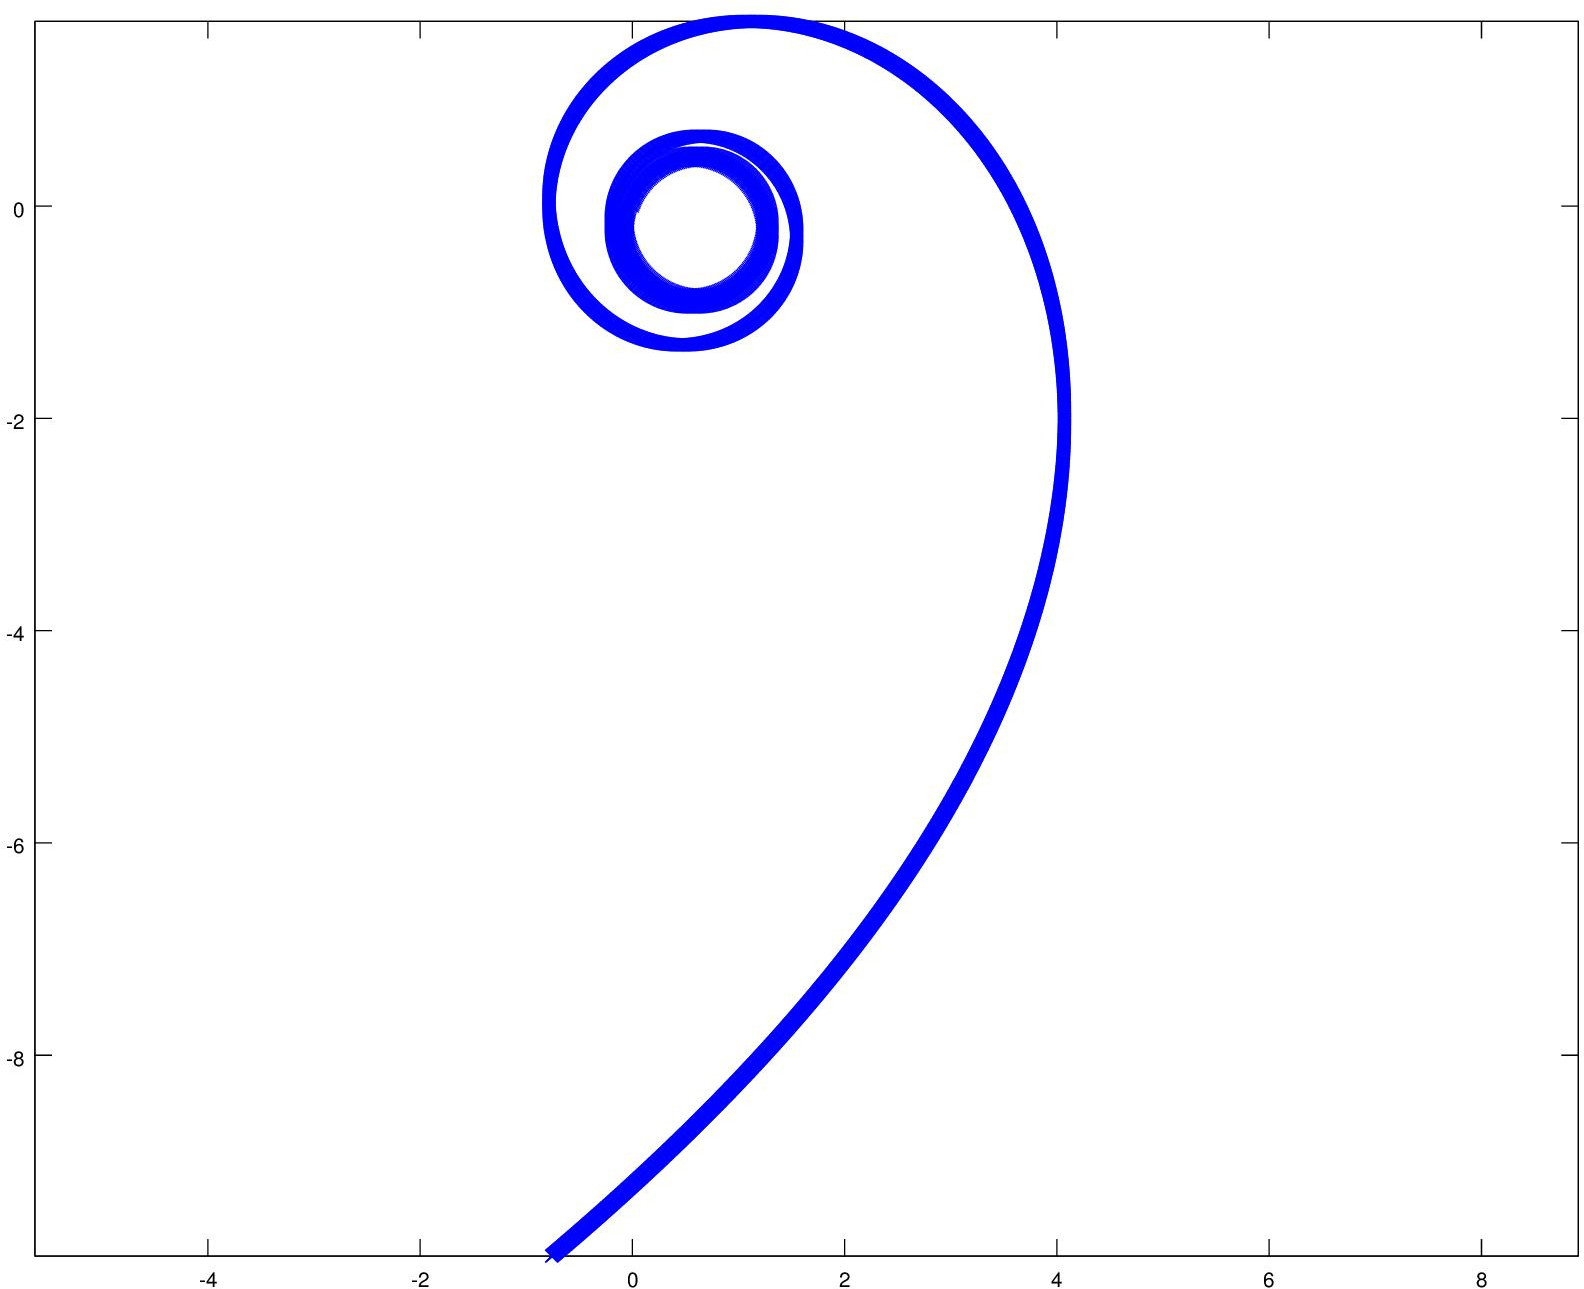
\includegraphics[width=0.5\textwidth]{images/traverse_spiral.jpg}
	\caption{Omni-Robot Traversing a Spiral}
	\label{fig:omni_robot_spiral}
\end{figure}






\newpage
\section{Measurement Model}
\label{sec:measurement_model}

Lets suppose the robot has a GPS and magnometer sensor. It is given that ``The
GPS output is in true North, East (and Down, not used here) and the
magnetometer points to magnetic north (your declination is 9.7 degrees West in
Waterloo, ON). Define additive noise distributions, with standard deviations in
North and East of 0.50m, and in magnetic north of 10 degrees.''

Given the above information, our measurement noise covariance matrix $Q$ is:

\begin{equation}
	Q = 
	\begin{bmatrix}
		0.5 & 0 & 0 \\
		0 & 0.5 & 0 \\
		0 & 0 & 10		
	\end{bmatrix}
\end{equation}

With a mean $\mu$ of:

\begin{equation}
	\mu = 
	\begin{bmatrix}
		0 \\
		0 \\
		-0.1692 
	\end{bmatrix}
\end{equation}

Note that 9.7 degrees is 0.1692 radians. Now that we have $\mu$ and $Q$, the 
Gaussian Additive Noise then becomes:

\begin{equation}
	\delta_{t} \sim \mathcal{N} (\mu, Q)
\end{equation}

To complete the measurement model it becomes:

\begin{align}
	y(t) &= C(t) x(t) + \delta_{t} \\
	&=
	\begin{bmatrix}
		1 & 0 & 0 \\
		0 & 1 & 0 \\
		0 & 0 & 1
	\end{bmatrix}
	\begin{bmatrix}
		x \\
		y \\
		\theta 
	\end{bmatrix}
	+
	\delta_{t}
\end{align}




\newpage
\section{Defining the Extended Kalman Filter for the Omni-directional Robot}
\label{sec:ekf_defintion}

The Extended Kalman filter (EKF) has two stages, the prediction and measurement 
updates. To complete the EKF we need to linearize the motion and measurement 
model, we detail that in the following sections.

\subsection{Linearizing the Motion Model}
\label{subsec:ekf_motion_model_linearization}
Normally if our motion model and/or measurement model is linear we can simply 
use the Kalman Filter, however in the non-linear case we have to use the 
Extended Kalman Filter (EKF). In our case we have to linearize the non-linear 
motion model $g(x_{t-1}, u_{t})$ using 1st order Taylor Series Expansion:

\begin{align}
	g(x_{t-1}, u_{t}) 
	& \approx 	
		g(\mu_{t - 1}, u_{t}) 
			+ \dfrac{\partial g(x_{t-1}, u_{t})}{x_{t - 1}} 
				\bigg|_{x_{t - 1} = \mu_{t - 1}}
			(x_{t - 1} - \mu_{t - 1}) \\
	& = g(\mu_{t - 1}, u_{t}) + G_{t} \cdot (x_{t - 1} - \mu_{t - 1})
\end{align}

Where $G_{t}$ is the first order differential of the non-linear motion model. 
We have, however, omitted the differentiation because we already know what 
$G_{t}$ is, since we have already derived the differential of $g(x_{t-1}, 
u_{t})$ in Section~\ref{sec:motion_model_derivation}.

\begin{equation}
	G_{t} = \dot{g}(\theta, \omega) = R(\theta)^{-1} J_{1}^{-1} J_{2} \omega
\end{equation}

Where $R(\theta)$, $J_{1}$, $J_{2}$ and $\omega$ are (derived in 
Section~\ref{sec:motion_model_derivation}): 

\begin{align}
	R(\theta) &= 
 	\begin{bmatrix}
	    \cos{(\theta)} & -\sin{(\theta)} & 0 \\
	    \sin{(\theta)} & \cos{(\theta)} & 0 \\
	    0 & 0 & 1
    \end{bmatrix} \\
	J_{1} &= 
	\begin{bmatrix}
			0 & 1 & l \\
  	    	-\cos(\frac{\pi}{6}) & -\sin(\frac{\pi}{6}) & l \\
   	    	\cos(\frac{\pi}{6}) & -\sin(\frac{\pi}{6}) & l
    \end{bmatrix} \\
    J_{2} &=
    \begin{bmatrix}
        r & 0 & 0 \\
        0 & r & 0 \\
        0 & 0 & r
    \end{bmatrix} \\
    \omega &= 
	    \begin{bmatrix}
	       \omega_{1} \\
	       \omega_{2} \\
	       \omega_{3} \\
	    \end{bmatrix}
\end{align}

\begin{equation}
	G_{t} = \dot{g}(\theta, \omega) =
	\begin{bmatrix}
		\frac{2}{3} \sin(\theta) r \omega_{1}
			- \frac{1}{\sqrt{3}} \cos(\theta) r \omega_{2}
				- \frac{1}{3} \sin(\theta) r \omega_{2}
			+ \frac{1}{\sqrt{3}} \cos(\theta) r \omega_{3}
				- \frac{1}{3} \sin(\theta) r \omega_{3} \\ \\
		\frac{2}{3} \cos(\theta) r \omega_{1}
			+ \frac{1}{\sqrt{3}} \sin(\theta) r \omega_{2}
				-\frac{1}{3} \cos(\theta)r \omega_{2}
			- \frac{1}{\sqrt{3}} \sin(\theta) r \omega_{3}
				-\frac{1}{3} \cos(\theta) r \omega_{3} \\ \\
		\frac{1}{3l} r \omega_{1}
			+ \frac{1}{3l} r \omega_{2}
			+ \frac{1}{3l} r \omega_{3}
	\end{bmatrix}
\end{equation}



\newpage
\subsection{Linearizing the Measurement Model}
\label{subsec:ekf_measurement_model_linearization}

As for the measurement model, it does not require linearization since in 
Section~\ref{sec:measurement_model} we derived a linear measurement model. 
Therefore $H_{t} = C_{t}$.

\begin{equation}
	H_{t} = C_{t} = 
	\begin{bmatrix}
		1 & 0 & 0 \\
		0 & 1 & 0 \\
		0 & 0 & 1
	\end{bmatrix}
\end{equation}



\subsection{Summary}
\label{subsec:ekf_def_summary}

Now that we have defined what $g(x_{t - 1})$, $G_{t}$ and $H_{t}$ (along with
 intial values for the states) we have enough information to incorporate them
  into the EKF model.



\newpage
\section{Implementing the Extended Kalman Filter}

In the EKF we have used the following values:

\begin{align*}
	\mu_{0} &= 
		\begin{bmatrix}
			0 \\
			0 \\
			0
		\end{bmatrix} \\
	u_{0} &= 
	\begin{bmatrix}
		-15.5 \\
		-10.5 \\
		1.5
	\end{bmatrix} \\
	H_{t} &=
	\begin{bmatrix}
		1 & 0 & 0 \\
		0 & 1 & 0 \\
		0 & 0 & 1
	\end{bmatrix} \\
	G_{t} &= \dot{g}(\theta, \omega) \\
		&= R(\theta)^{-1} J_{1}^{-1} J_{2} \omega
	    \begin{bmatrix}
	        \dot{x} \\
	        \dot{y} \\
	        \dot{\theta}
	    \end{bmatrix} \\
	    &= 
	        \begin{bmatrix}
		        \cos{(\theta)} & -\sin{(\theta)} & 0 \\
		        \sin{(\theta)} & \cos{(\theta)} & 0 \\
		        0 & 0 & 1
	        \end{bmatrix}^{-1}
	        \begin{bmatrix}
	            0 & 1 & l \\
	          	-\cos(\frac{\pi}{6}) & -\sin(\frac{\pi}{6}) & l \\
	        	\cos(\frac{\pi}{6}) & -\sin(\frac{\pi}{6}) & l
	        \end{bmatrix}^{-1}
	        \begin{bmatrix}
	            r & 0 & 0 \\
	            0 & r & 0 \\
	            0 & 0 & r
	        \end{bmatrix}
		    \begin{bmatrix}
		       \omega_{1} \\
		       \omega_{2} \\
		       \omega_{3} \\
		    \end{bmatrix} \\
\end{align*}


\end{document}